\section{Versuchsaufbau: LEP und OPAL}
Im Versuch werden Daten ausgewertet, die in den Jahren 1989 bis 2000 am
CERN\footnote{Conseil Européen pour la Recherche Nucléaire} während des
LEP\footnote{Large Electron-Positron Collider}-Experiments gewonnen wurden.
In dem 27\,km langen Tunnel des Teilchenbeschleunigers kreisten gegenläufig Pakete von Elektronen und Positronen
und kollidierten an vier Stellen im Strahl \cite{manual}.
An jeder der vier Wechselwirkungszonen stand ein Detektor, einer davon war der
OPAL\footnote{Omni Purpose Apparatus at LEP}-Detektor.
Der Aufbau dieses Detektors wird im Folgenden beschrieben.

\begin{figure}[H]
\begin{center}
  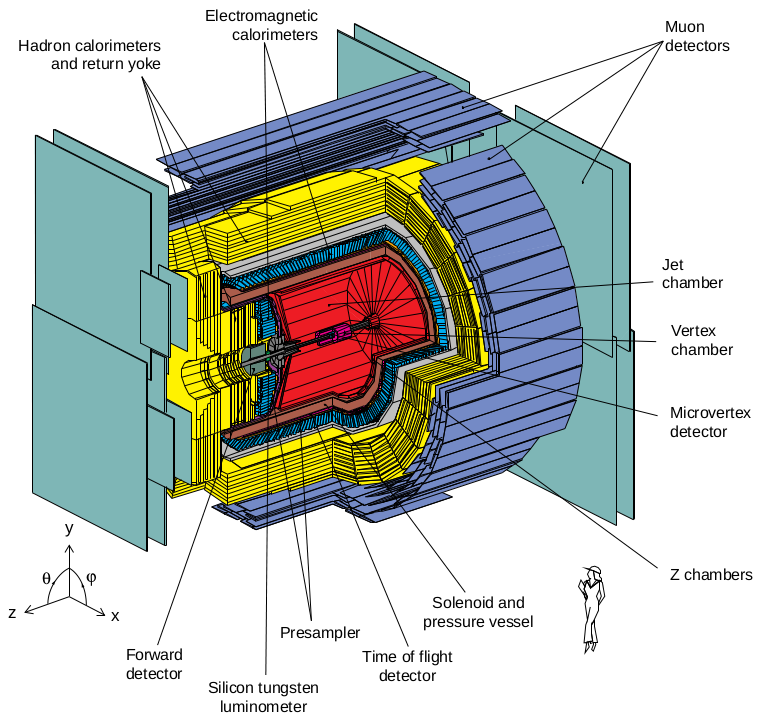
\includegraphics[width=\textwidth]{../img/aufbau.png}
  \caption{Aufbau des OPAL-Detektors am LEP (aus \cite{manualmuc}).}
  \label{img:aufbau}
\end{center}
\end{figure} 

\begin{figure}[H]
\begin{center}
  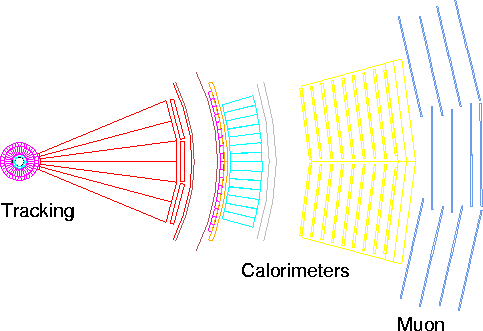
\includegraphics[width=0.6\textwidth]{../img/opalslice_tr.png}
  \caption{Schematischer Schnitt durch den OPAL-Detektor senkrecht zum \ee-Strahl.}
  \label{img:schnitt}
\end{center}
\end{figure} 


LEP\\
OPAL \\
Aufbau \\
Beschreibung der verschiedenen Detektoren 